\documentclass[]{article}

\usepackage[utf8]{inputenc}

\usepackage[T1]{fontenc}

\usepackage[english]{babel}

\usepackage{amsmath, amsfonts, amssymb, amsthm}

\usepackage{fullpage}

\usepackage{enumerate}
\usepackage{graphicx}
\usepackage{algorithm}
\usepackage{algorithmic}

\usepackage{hyperref}
\hypersetup{
    colorlinks,
    citecolor=black,
    filecolor=black,
    linkcolor=black,
    urlcolor=black
}


%Pour les algos
\floatname{algorithm}{Algorithme}
\renewcommand{\algorithmicrequire}{\textbf{Entrée:}}
\renewcommand{\algorithmicensure}{\textbf{Sortie:}}
\renewcommand{\algorithmicif}{\textbf{si}}
\renewcommand{\algorithmicthen}{\textbf{alors}}
\renewcommand{\algorithmicelse}{\textbf{sinon}}

\title{
{\Huge Digital filtering}\\
Signal processing\\
}

\author{
\textbf{Dell’Aria Doriano}\\
\and
\textbf{Goffaux Lionel}
}


\date{\today\\
Academic Year 2020-2021\\
Bachelor's degree in Computer Science}

\begin{document}

\maketitle

\section{Approximation of second order filters}
\subsection*{Band-pass filter:}
\begin{enumerate}
    \item Find $\theta$ : we compute $\theta = \frac{f}{2\pi}Fe = 1.88$.
    \item Find $\rho$ : we set K = 1 and we draw this graph representing the height difference between \{120Hz,121Hz\} and \{119Hz,120Hz\}.
    \begin{figure}[H]
        \centering
        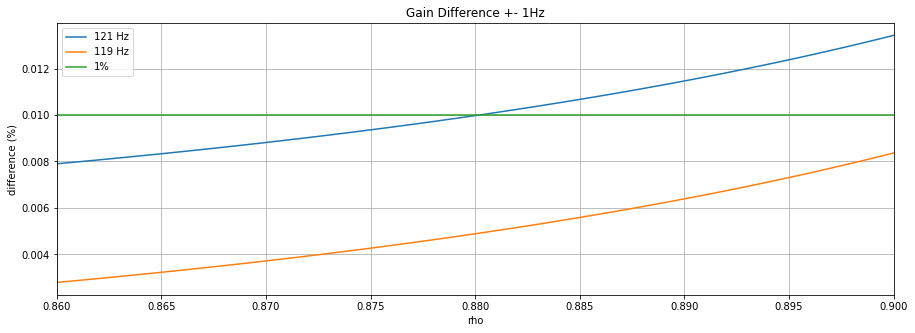
\includegraphics[scale=0.5]{q11.png}
    \end{figure}
    we set $\rho$ = 0.87
    \item Find K : we compute $K = \frac{1}{A_{120Hz}}=0.2432$.
\end{enumerate}
The transfer function of the pass-band filter is 
$$H(Z) = K\frac{1 - \cos{(\theta)} Z^{-1}}{1 - 2\rho \cos{(\theta)Z^{-1} +\rho^2Z^{-2}}}$$
where K = 0.2432, $\rho$ = 0.87 and $\theta$ = 1.88. The frequency response as well as the poles and zeros position of this filter are the following.

\begin{figure}[H]
    \centering
    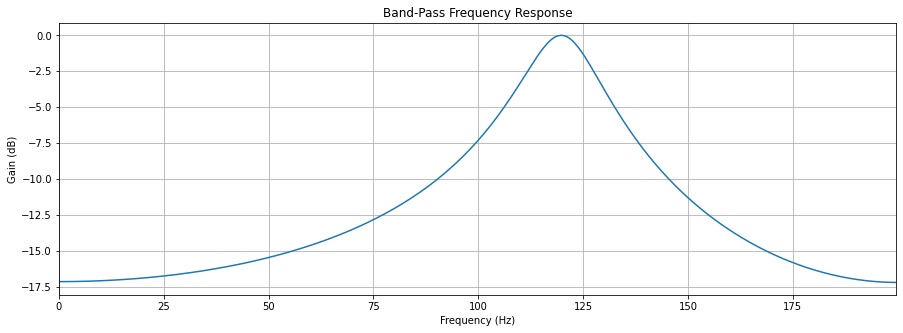
\includegraphics[scale=0.5]{q12.png}
\end{figure}

\begin{figure}[H]
    \centering
    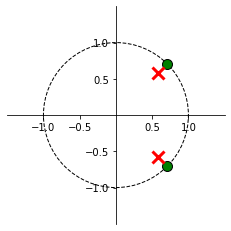
\includegraphics[scale=0.7]{q17.png}
\end{figure}


\subsection*{Band-stop filter:}
\begin{enumerate}
    \item Find $\theta$ : we compute $\theta = \frac{50}{2\pi}Fe = 0.78$.
    \item Find $\rho$ : we set K = 1 and we draw this graph representing the attenuation at 49.9 Hz and 50.1 Hz. 
    We want to attenuate these frequencies at -47dB.
    \begin{figure}[h]
        \centering
        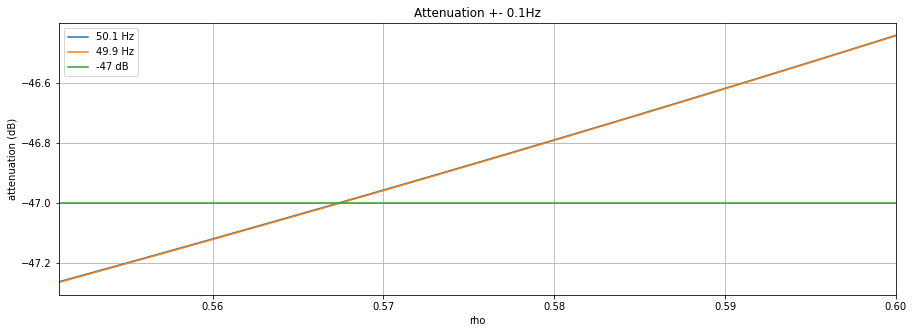
\includegraphics[scale=0.5]{q13.png}
    \end{figure}\\
    We set $\rho = 0.56$.
    \item Find K : we computed $K = \frac{1}{A_{120Hz}}=0.6713$.
\end{enumerate}
The transfer function of the stop-band filter is 
$$H(Z) = K\frac{1 - 2\cos{(\theta)} Z^{-1} + Z^{-2}}{1 - 2\rho \cos{(\theta)Z^{-1} +\rho^2Z^{-2}}}$$
where K = 0.6714, $\rho$ = 0.56 and $\theta$ = 0.78. The frequency response as well as the poles and zeros position corresponding are the following.

\begin{figure}[H]
    \centering
    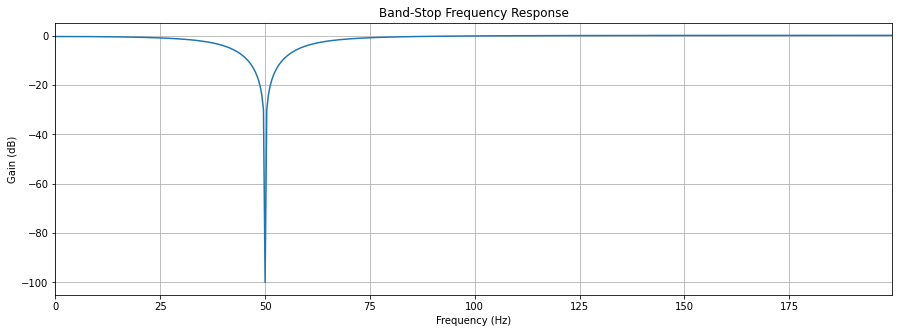
\includegraphics[scale=0.5]{q14.png}
\end{figure}

\begin{figure}[H]
    \centering
    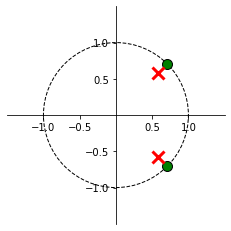
\includegraphics[scale=0.7]{q17.png}
\end{figure}

\pagebreak

\subsection*{Band-pass + band-stop filter}

Now we can add these two filters together and plot their frequency response. 
The poles and zeros position of this new filter is exactly the same as the two previous ones together.

\begin{figure}[H]
    \centering
    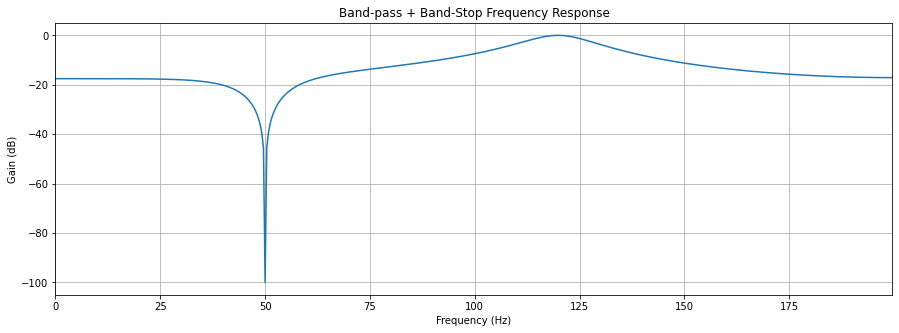
\includegraphics[scale=0.5]{q15.png}
\end{figure}

\begin{figure}[H]
    \centering
    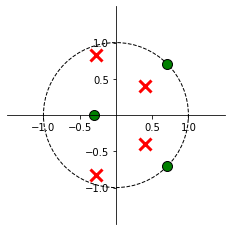
\includegraphics[scale=0.7]{q18.png}
\end{figure}

\pagebreak

\section{Approximation of higher order filters}

\subsection*{Recursive filter}

We see that the specifications are respected.
These specifications are drawn in green on the graph.

\begin{figure}[H]
    \centering
    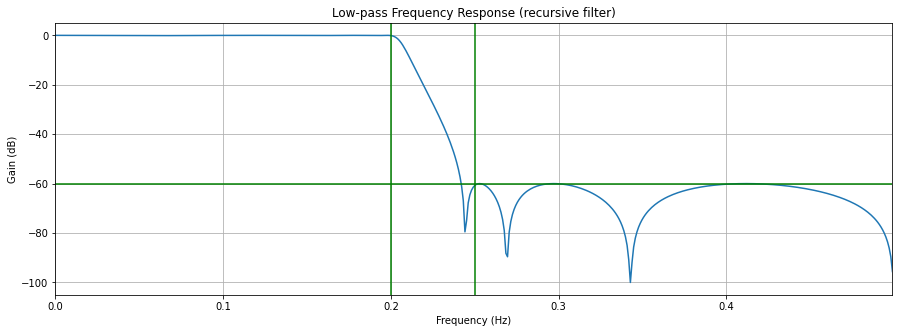
\includegraphics[scale=0.5]{q21.png}
\end{figure}

\begin{figure}[H]
    \centering
    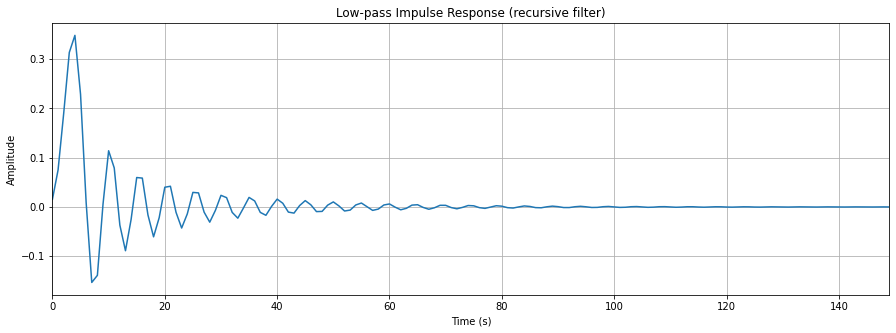
\includegraphics[scale=0.5]{q22.png}
\end{figure}

\begin{figure}[H]
    \centering
    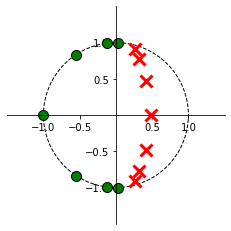
\includegraphics[scale=0.7]{q23.png}
\end{figure}


\subsection*{Non-recursive filter}

We also see that the specifications are respected.
These specifications are drawn in green on the graph.

\begin{figure}[H]
    \centering
    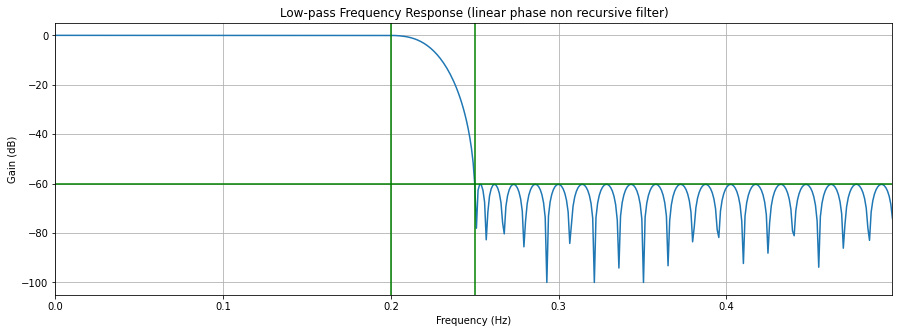
\includegraphics[scale=0.5]{q24.png}
\end{figure}

\begin{figure}[H]
    \centering
    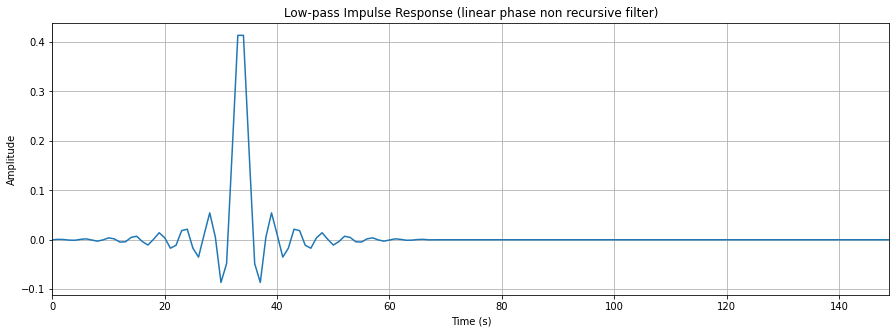
\includegraphics[scale=0.5]{q25.png}
\end{figure}

\begin{figure}[H]
    \centering
    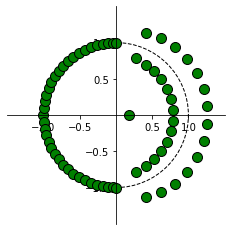
\includegraphics[scale=0.7]{q26.png}
\end{figure}

\subsection*{Comparison between the two filters}

For the recursive one, we compute a 7th-order filter and a 68th-order filter for the non-recursive one.
We estimate the number of computations to be twice filter's order. So, for the recursive filter
we have 14 operations per samples and 136 for the non-recursive one.

\end{document}